%===============================================================================
% $Id: ifacconf.tex 19 2011-10-27 09:32:13Z jpuente $  
% Template for IFAC meeting papers
% Copyright (c) 2007-2008 International Federation of Automatic Control
%===============================================================================
\documentclass{ifacconf}

\usepackage{graphicx}      % include this line if your document contains figures
\usepackage{natbib}        % required for bibliography
\usepackage{hyperref}
\usepackage{amsmath,amssymb}
\usepackage{mathtools} % for matrix left-alignment

% real and imaginary symbols
\renewcommand{\Re}{\operatorname{\mathbb{R}e}}
\renewcommand{\Im}{\operatorname{\mathbb{I}m}}
%===============================================================================
\begin{document}
\begin{frontmatter}

\title{Force-Limited Control of Wave Energy Converters using a Describing Function Linearization\thanksref{footnoteinfo}} 
% Title, preferably not more than 10 words.

\thanks[footnoteinfo]{This material is based upon work supported by the National Science Foundation Graduate Research Fellowship under Grant No. DGE–2139899.}

\author[First]{Rebecca McCabe} 
\author[Second]{Maha N. Haji} 
\address*{Sibley School of Mechanical and Aerospace Engineering, Cornell University, 
   Ithaca, NY 14853 USA }
   \address[First]{e-mail: rgm222@cornell.edu}
   \address[Second]{e-mail: maha@cornell.edu}

\begin{abstract}                % Abstract of not more than 250 words.
Actuator saturation is a common nonlinearity in physical systems. In wave energy conversion, force saturation can be a convenient way to limit the size and cost of the generator and the mechanical loading on the drivetrain with minimal impact on energy generation. However, such nonlinear dynamics typically demand numerical time-domain simulation rather than analytical frequency-domain analysis, which increases computational cost and diminishes designer intuition. This paper proposes the use of describing functions to accurately linearize the force saturation dynamics and stay in the frequency domain. It explores the impact of the force limit on electrical power production of a generic single degree of freedom wave energy converter under energy-maximizing impedance control. Analytical expressions are obtained and the Smith chart is used as a visualization tool. The expressions are nondimensionalized to quantify the effect of the maximum force value on devices with different hydrodynamics and powertrain dynamics. Systems with predominately real-valued mechanical impedances are less sensitive to force limits than their more reactive counterparts. Sensitivity results are discussed in the context of sizing drivetrain components such as the generator, while the results can also apply to explore the impact of controller bandwidth and parameter error. The describing function method is over 200 times faster than a time-domain simulation,
%and X times faster than a spectral-domain simulation
showing promise as a technique to enable future studies such as large-scale design optimization and control co-design.
\end{abstract}

\begin{keyword}
Constrained control, control of renewable energy resources, systems with saturation, nonlinear and optimal marine system control, sensors and actuators.
\end{keyword}

\end{frontmatter}
%===============================================================================

\section{Introduction}
\subsection{Motivation}
Ocean wave energy converters are an immature yet promising source of renewable energy to decarbonize coastal electricity grids and small offshore systems. Due to waves' high-force, low-speed nature, sizing the device to collect maximum energy can lead to large structural and powertrain forces that ultimately reduce the system's economic viability. Wave Energy Converters (WECs) benefit from controllers that maximize power while obeying force constraints, although the resulting nonlinearity muddies intuition and increases computational cost. This paper examines the tradeoff of maximum force with power production using describing functions, a technique which is intuitive, analytical, and linear. This enables computational efficiency, the opportunity to apply linear system analysis tools, and the ability to couple with other models to perform multidisciplinary design optimization or control co-design in the future. The results equally apply to other types of impedance mismatch such as controller bandwidth limitations and parameter errors.

\subsection{Literature Review}
Existing work on powertrain constraints in wave energy conversion is predominately in numerical constrained optimal control, typically using either model predictive control or spectral/pseudo-spectral methods.  \cite{strofer_control_2023} implement a force constraint in the pseudo-spectral toolbox WecOptTool and optimizes the controller gains and drivetrain impedance. \cite{pena-sanchez_control_2022} utilize a pseudo-spectral method with simultaneous force and position constraints to perform economic optimization of the generator sizing.  \cite{sichani_constrained_2014} sweep the value of a force constraint numerically and shows that the optimal damping gets higher as the force constraint lowers, while the optimal stiffness changes only slightly. \cite{tom_pseudo-spectral_2017} use a pseudo-spectral method with pitch amplitude and torque constraints, while also including a force term in the objective. \cite{faedo_optimal_2017} review model predictive control for WECs and notes constraints related to position, velocity, force, rate of change of force, and power flow direction (passivity).

A minority of work tackles the problem analytically. \cite{zou_optimal_2017} use the Pontryagin maximum principle to show that a bang-singular arc-bang controller is optimal, revealing that saturating the unsaturated optimal solution can still be optimal in certain cases, while \cite{abdulkadir_optimal_2024} have  extended the result to arrays. Both of these papers yield analytical piecewise expressions for the optimal control force, but finding the full state trajectory including the power still requires numerical simulation. %(as far as I could see? double check this) -
\cite{bacelli_geometric_2013} present a geometric tool to analyze simultaneous force and position constraints. The technique uses a spectral method (Galerkin's method) but needs to approximate constraints with their 2-norm, effectively constraining the root-mean-square of the signal rather than the peak. \cite{merigaud_geometrical_2023} likewise introduce a geometric tool, this one only accounting for motion amplitude constraints and focusing more on the hydrodynamics than the powertrain. The tool is visually and mathematically similar to a Smith chart. To the authors' knowledge, no one in the wave energy space has used describing functions to address constraints, although \cite{flower_describing-function_1980} utilize describing functions to model a WEC with friction-like nonlinear powertrain damping. Outside of the wave energy field, \cite{fukui_impedance_2021} have applied describing functions to model velocity saturation and torque saturation on a two-motor impedance-controlled system for a robotics application, and experimentally validate the results.

%- Babarit 2023 PTO capping: effect of 3 different force caps and 3 different power caps on the energy spectrum, with energy calculated from real sea data in 4 different ways. The focus is not on the energy but on the accuracy of the energy prediction in different calculation methods. \cite{de_la_torre-castro_combined_2023}
% - Many people doing MPC with constraints
% - Tedeschi 2011 power saturation with simulink \cite{tedeschi_effect_2011}
% - Dan Herber 2014 \cite{herber_wave_2014}

% STILL NEED TO CHECK
% - Giorgio's paper that implements constraints for a real WEC (+thesis?)
% - Ringwood follow on paper for pneumatic valve

\subsection{Paper Contribution and Outline}
Wave energy converters are designed to resonate with incoming waves, and maximum power transfer requires impedance matching of the powertrain, controller, and hydrodynamic body. However, perfect impedance matching may not be possible in some conditions due to plant uncertainties, controller bandwidth, and actuator limitations. In this sense, force saturation can be seen as an impedance mismatch. Therefore, before analyzing the nonlinear dynamics of saturation, it is first informative to examine the properties of an impedance-mismatched linear system. This is outlined and visualized in section~\ref{sec:linear}, starting for a general system and then moving to the specific dynamics of an oscillating-body wave energy converter with an electric generator. In section~\ref{sec:nonlinear}, the describing function is introduced to handle the saturation nonlinearity, providing an intuitive linear approximation. Sensitivity results are provided in section~\ref{sec:sensitivities}, focusing on implications in powertrain sizing.

\section{Peak Limiting in the Linear Case}\label{sec:linear}
\subsection{General Impedance-Matched System}
The analysis starts with a generic linear system modeled as a Thévenin equivalent circuit with AC voltage source $V_{th}$ and complex source impedance $Z_{th}$, shown in Fig.~\ref{fig:circuit}.
\begin{figure}
\begin{center}
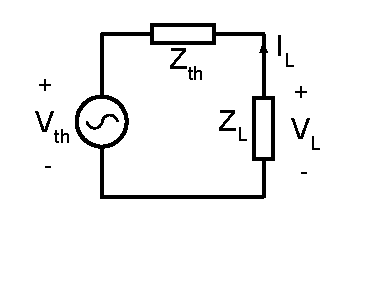
\includegraphics[width=6cm]{ifacconf_latex/figs/IFAC CAMS Circuit drawing.pdf}    % The printed column width is 8.4 cm.
\caption{Thévenin equivalent circuit for linear system} 
\label{fig:circuit}
\end{center}
\end{figure}
The load impedance $Z_L$ is to be selected, with the conflicting goals of maximizing average power transfer $\overline{P}_L$ and minimizing the peak amplitude of load current $|I_L|$ or voltage $|V_L|$. Maximum power transfer occurs when there is impedance matching, meaning $Z_L = Z_{th}^*$ where $*$ indicates the complex conjugate. The load average power, peak voltage, and peak current at this matched point, denoted $\overline{P}_L^m, |V_L^m|,$ and $|I_L^m|$ respectively, are found as
\begin{equation}\label{eq:matched-values}
    \overline{P}_L^m = \frac{|V_{th}|^2}{8 \Re(Z_{th})}, 
    |V_L^m| = \frac{|V_{th}| |Z_{th}|} {2 \Re(Z_{th})}, 
    |I_L^m| = \frac{|V_{th}|}{2 \Re(Z_{th})}
\end{equation}

To consider all possibilities of the unmatched case, we set $Z_L = z Z_{th}^*$ for arbitrary complex number $z$. The space of $z$ can be visualized using a Smith chart, where $\Re(z)$ is on a curved horizontal axis and $\Im(z)$ is on a curved vertical axis. The axes are curved such that the chart can be simultaneously read as a standard polar plot of the complex reflection coefficient $\Gamma$, which is a transformation of $z$ defined as $\Gamma = \frac{z-1}{z+1}$. The impedance-matched case of $z=1$, $\Gamma = 0$ is found at the center of the plot, the minimum voltage at $z=0$, $\Gamma = -1$ on the left, and the minimum current at $z \rightarrow \infty$, $\Gamma = 1$ on the right.

In the unmatched case, the average power, peak voltage, and peak current can be found using standard circuit techniques and expressed as fractions of their matched counterparts. The power ratio is:
\begin{equation}\label{eq:ratio-power}
     \frac{\overline{P}_L}{\overline{P}_L^m} = 1 - |\Gamma|^2
\end{equation}
\begin{figure}[bp!]
    \centering
    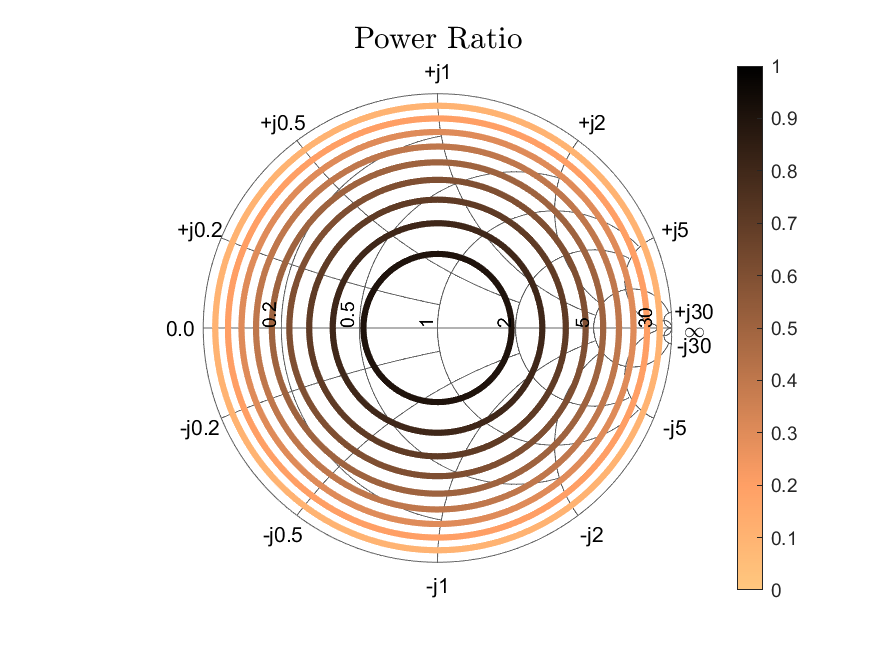
\includegraphics[width=\linewidth]{ifacconf_latex/figs/power-smith.png}
    \caption{Smith chart representing the average power at the load for any $z=\frac{Z_L}{Z_{th}^*}$, using the expression (\ref{eq:ratio-power}). The real part of $z$ is plotted on the arcs labeled horizontally, while the imaginary part is plotted on the arcs labeled radially along the outside of the chart. The reflection coefficient $\Gamma$ is also represented as a polar plot centered at $z=1$.}
    \label{fig:power-smith}
\end{figure}
\begin{figure*}[tb!]
    \centering
    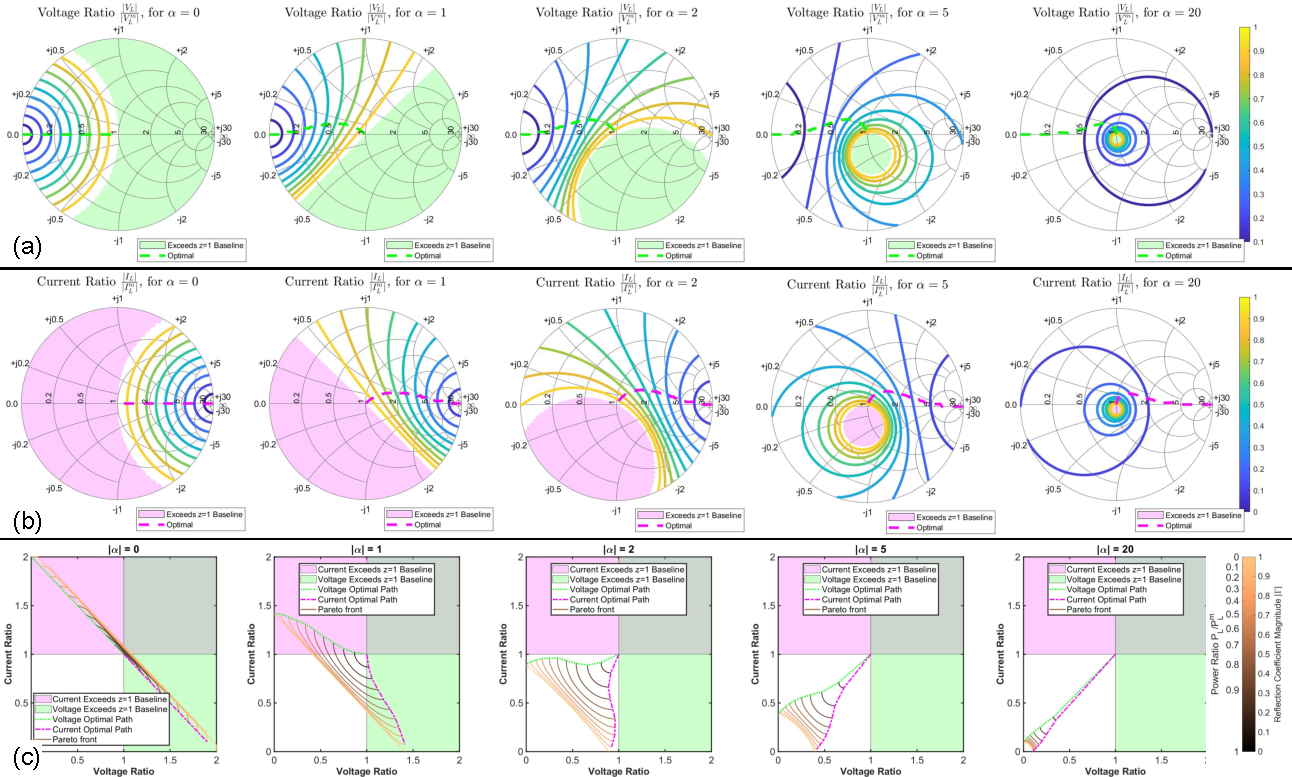
\includegraphics[width=18.2cm]{ifacconf_latex/figs/IFAC CAMS paretos (2).pdf}
    \caption{Smith charts representing the (a) peak voltage and (b) peak current at the load for any $z=\frac{Z_L}{Z_{th}}$, paired with (c) the pareto tradeoff between voltage, current, and power. The parameter $\alpha$ is swept, representing the relative reactance of the Thévenin impedance $Z_{th}$. Shaded regions indicate that the voltage (green) or current (pink) ratios exceed one. Dashed lines indicate the optimal contours.}
    \label{fig:ratio-smith}
\end{figure*}
This relationship is visualized on the Smith chart in Fig.~\ref{fig:power-smith}. As the impedance ratio $z$ gets further away from the impedance-matched condition $z=1$ at the center of the circle, the power lowers quadratically.

The corresponding voltage and current ratios are:
\begin{equation}\label{eq:ratios}
\begin{aligned}
    \frac{|V_L|}{|V_L^m|} &= \sqrt{\frac{|\Gamma|^2 + 2 \Re(\Gamma) + 1}{\alpha^2 |\Gamma|^2 + 2 \alpha \Im(\Gamma) + 1} } \\
     \frac{|I_L|}{|I_L^m|} &= \sqrt{\frac{|\Gamma|^2 - 2 \Re(\Gamma) + 1}{\alpha^2 |\Gamma|^2 + 2 \alpha \Im(\Gamma) + 1} }\\
\end{aligned}
\end{equation}

The voltage and current relationships in (\ref{eq:ratios}) depend not only on $\Gamma$ but also on the phase of $Z_{th}$ via the parameter $\alpha = \frac{\Im(Z_{th})}{\Re(Z_{th})}$. These relationships are visualized on the Smith charts in Fig.~\ref{fig:ratio-smith}.

Only positive $\alpha$ (inductive $Z_{th}$) are shown for brevity. The contours for negative $\alpha$ (capacitive $Z_{th}$) can be found by reflecting the graphs over the horizontal axis ($\Im(\Gamma) = 0)$ due to symmerty. On the Smith charts, points where the voltage and current ratios exceed 1 are shaded. These points are undesirable because they absorb less power than the baseline $z=1$, $\Gamma=0$ matched case while having higher peaks. The optimal contours (highest voltage and current ratios, $\frac{|V_L|}{|V_L^m|}$ and $\frac{|I_L|}{|I_L^m|}$, for a given power ratio $\frac{\overline{P}_L}{\overline{P}_L^m}$) are traced out with dashed lines. This optimal tradeoff $(\cdot)^\textrm{opt}$ can be found analytically by setting the partial derivative of $\frac{|V_L|}{|V_L^m|}$ and $\frac{|I_L|}{|I_L^m|}$ with respect to $\angle\, \Gamma$ equal to zero, where $\angle\, \Gamma= \tan^{-1} \frac{\Im(\Gamma)}{\Re(\Gamma)}$. This results in
\begin{equation}\label{eq:optimal-vi}
\begin{aligned}
    %\frac{|V_L|}{|V_L^m|}^\textrm{opt} &= 2 \tan^{-1}{ \frac{\alpha^2 |\Gamma|^2 - \sqrt{(\alpha^2 + 1)(\alpha^2 |\Gamma|^4 + 1)} + 1}{\alpha (1 - |\Gamma|)^2}} \\
\hspace{-8pt} \frac{|V_L|}{|V_L^m|}^\textrm{opt} \hspace{-13pt}= \frac{|I_L|}{|I_L^m|}^\textrm{opt} \hspace{-13pt}&= 2 \tan^{-1}{ \frac{\alpha^2 |\Gamma|^2 - \sqrt{(\alpha^2 + 1)(\alpha^2 |\Gamma|^4 + 1)} + 1}{\alpha (1 + |\Gamma|)^2}}
\end{aligned}
\end{equation}

These optimal contours are aggregated in Fig.~\ref{fig:pareto} to show the tradeoff between power and voltage/current. Interestingly, as $|\alpha|$ grows (i.e., as $Z_{th}$ becomes less resistive and more reactive), there is less of a power penalty for a given voltage or current reduction. In other words, the power in the pure resistive $Z_{th}$ case is the most sensitive to voltage and current limits. If the goal is to obey a current limit $|I_L| \leq I_{max}$ without regard for the voltage, then the optimal solution from Fig.~\ref{fig:pareto} is expressed as:
\begin{equation}
   \frac{\alpha^2 |\Gamma|^2 - \sqrt{(\alpha^2 + 1)(\alpha^2 |\Gamma|^4 + 1)} + 1}{\alpha (1 + |\Gamma|)^2} \leq \tan \frac{\Re(Z_{th}) I_{max}}{|V_{th}|}
\end{equation}
%Furthermore, the curves for the optimal voltage and current ratios align almost exactly. The sign difference on $|\Gamma|$ in the denominator has minimal effect at $|\Gamma|\rightarrow 0$, and also has minimal effect at $|\Gamma|\rightarrow 1$ because the numerator approaches zero.
\begin{figure}
    \centering
    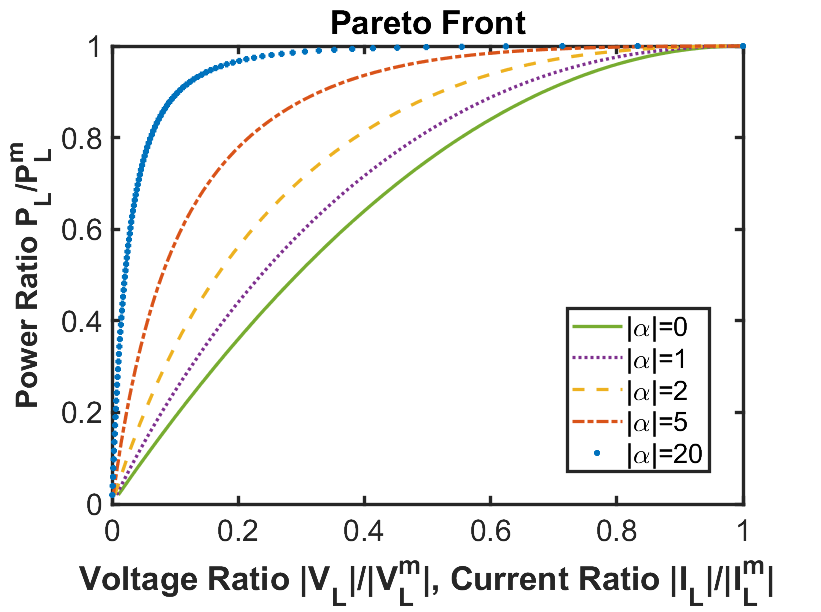
\includegraphics[width=\linewidth]{ifacconf_latex/figs/pareto2.png}
    \caption{Pareto front for optimal voltage and current ratios.}
    \label{fig:pareto}
\end{figure}
Note that some of the optimal contours require a $z$ with nonzero imaginary part, i.e. a $Z_L$ that is more or less reactive than the impedance-matched case, rather than merely scaled up or down. Here it is worth discussing the difference between ``constrained optimal control" and ``optimal constrained control." The former refers to the unconstrained optimal controller that has been scaled or saturated until it meets the constraint, while the latter refers to the controller that is optimal for the constrained problem, which may be distinct. Scaling or saturating the control signal computed with the unconstrained optimal impedance (z = 1) yields a signal with a fundamental identical to one computed with a proportionally scaled linear controller impedance, effectively enforcing z to be a real number. This is distinct from the complex $z$ in the optimal profiles of (\ref{eq:optimal-vi}) and Fig.~\ref{fig:pareto}, which would be considered optimal constrained control. 

Furthermore, because the optimal voltage reduction path requires decreasing the impedance and the optimal current reduction path requires increasing the impedance, it is not possible to follow both paths simultaneously. For sufficiently high values of $|\alpha|$, it is possible to reduce both current and voltage simultaneously (i.e. avoid the shaded region of both Smith charts in Fig.~\ref{fig:ratio-smith} (a) and (b)), although for $\alpha=0$ a decrease in voltage is always associated with an increase in current and vice versa. This tradeoff is explored further in section (c) of Fig.~\ref{fig:ratio-smith}, a pareto front showing the nondominated combinations of the voltage, current, and power ratios.

These plots reveal the effect of an impedance mismatch on power, current, and voltage, and can be used to choose an appropriate load impedance based on the relative importance of power generation and peak limiting. The extent to which a given impedance mismatch decreases the current, voltage, and power is strongly dependent on the Thévenin impedance phase parameter $\alpha$, although we note that the baseline signal amplitudes in the matched case also depend implicitly on $\alpha$ through (\ref{eq:matched-values}).
% Considering a weighted linear objective function $J$ 

% \begin{equation}
%     J = a~ \frac{\overline{P}_L}{\overline{P}_L^m} - b~ \frac{|V_L|}{|V_L^m|} - (1 - a - b)~ \frac{|I_L|}{|I_L^m|}
% \end{equation}
% for $0 \leq a, b \leq 1$, we can substitute (\ref{eq:ratios}) and differentiate to derive the $\Gamma$ which maximizes $J$:

% \begin{equation}
%     \Gamma^\textrm{opt} = f(a, b, \alpha)
% \end{equation}
% This tradeoff is shown

% Note that substituting $a=1, b=0$ recovers the optimal current condition and $a=1, b=1$ the optimal voltage condition from (\ref{eq:optimal-vi}).

\subsection{Wave Energy Converters}
Applying the preceding analysis to a Wave Energy Converter (WEC) requires developing a Thévenin equivalent circuit for the WEC dynamics. We assume that the WEC consists of a floating body coupled to a power take-off (PTO) consisting of a drivetrain and a linear or rotational electric generator of the synchronous surface permanent magnet variety, although it is straightforward to substitute a hydraulic or other impedance provided the system remains linear. The generator is non-ideal, so the objective is electrical power, informed by the substantial differences when optimizing for mechanical versus electrical power which \cite{coe_useful_2023} summarize. The WEC dynamics in the frequency domain are:
\begin{equation}\label{eq:wec-dynamics}
\begin{aligned}
    &((m+A)s^2 + B_h s + K_h) X + F_{PTO} = F_e &&\textrm{Body}\\
    &G \tau_{PTO} = F_{PTO},~G s X = \Omega &&\textrm{Gear ratio}\\
    &\tau_{PTO} = (B_d + \frac{K_d}{s}) \Omega + \tau_{gen} &&\textrm{PTO}\\
    &\tau_{gen} = K_t I,~V = I(R + s L) - K_t \Omega &&\textrm{Generator}\\
    &V = (B_c + \frac{K_c}{s}) I &&\textrm{Controller}\\
    &P_{elec} = \frac{1}{2} \Re(I^* V) &&\textrm{Power}
\end{aligned}
\end{equation}
where $s=j\omega$ is the Laplace variable, $m$ is the mass, $A$ is the added mass, $B_h$ is the hydrodynamic damping, $K_h$ is the hydrostatic stiffness, $X$ is the WEC position, $F_{PTO}$ is the power take-off force, $F_e$ is the wave excitation force, $G$ is the gear ratio in a linear PTO or the inverse of the equivalent gear radius in a rotary PTO, $K_d$ and $B_d$ are the drivetrain mechanical stiffness and damping, $\tau_{gen}$ and $\Omega$ are the generator torque and rotational speed, $K_t$ is the generator torque constant, $I$ and $V$ are the generator q-axis current and voltage, $R$ and $L$ are the generator winding resistance and inductance, $K_c$ and $B_c$ are the controller stiffness and damping, and $P_{elec}$ is the average electrical power. While typically the controller is between $\tau_{gen}$ and $\Omega$, here the controller is assumed to act between voltage and current. This will result in different controller gains but provides equivalent dynamics and will make the definition of the relevant Thévenin equivalent more convenient. A block diagram of these dynamics is shown in Fig.~\ref{fig:block-diagram-dynamics}.
\begin{figure}
    \centering
    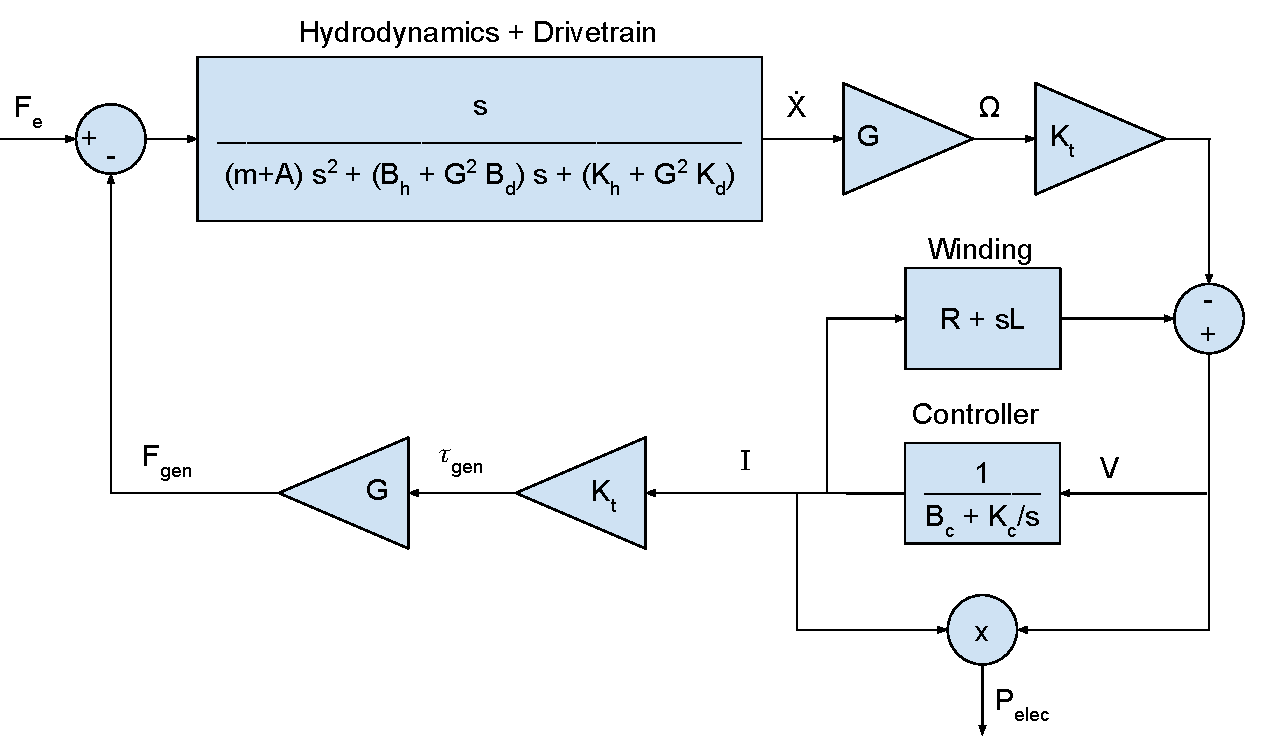
\includegraphics[width=\linewidth]{ifacconf_latex/figs/IFAC CAMS Dynamics Diagram - Electrical Control.pdf}
    \caption{Block diagram of dynamics.}
    \label{fig:block-diagram-dynamics}
\end{figure}
The hydrodynamic coefficients $A$ and $B_h$ are frequency dependent, but this dependence is omitted for notational convenience.

There are many ways to form a Thévenin equivalent circuit from these dynamics, depending on the desired line between the source and load impedance. Because we want to quantify electrical power rather than mechanical power, it makes sense to choose the controller as the load, $Z_L = Z_c = B_c + \frac{K_c}{s}$. This makes the Thévenin equivalent voltage correspond to generator q-axis voltage, $V_L = V$, and the Thévenin equivalent current correspond to generator q-axis current, $I_L = I$. With this choice, the Thévenin equivalent circuit parameters given by \cite{strofer_control_2023} are:
\begin{equation}\label{eq:thevenin}
\begin{aligned}
    Z_{th} &= Z_w + \frac{K_t^2 G^2}{Z_m} \\
    |V_{th}| &= \frac{K_t G F_e}{|Z_m|}
\end{aligned}
\end{equation}
where we have defined the winding impedance $Z_w = R + s L$ and the mechanical impedance $Z_m = B_h + G^2B_d + (m+A)s + \frac{K_h + G^2 K_d}{s}$.

From $Z_{th}$, we can derive $\alpha$ which relates to its phase and enables the practical interpretation of Fig.~\ref{fig:ratio-smith}:
\begin{equation}\label{eq:alpha}
    \alpha = \frac{\Im(Z_{th})}{\Re(Z_{th})} =  \frac{1+\Re(\frac{1}{\mathcal{Z}})}{\mathcal{L} + \Im(\frac{1}{\mathcal{Z}})}
\end{equation}
where $\mathcal{Z}$ and $\mathcal{L}$ represent the nondimensionalized mechanical impedance and inductance:
\begin{equation}
    \mathcal{Z} = \frac{RZ_m}{K_t^2G^2}, \quad
    \mathcal{L} = \frac{\omega L}{ R }
\end{equation}
noting that $\mathcal{L}$ is real while $\mathcal{Z}$ is complex. In most systems, $\mathcal{L} \approx 0$ because the wave period in the ocean is very slow compared to the electrical time constant of the winding. We previously saw that $|\alpha|$ greatly affects the sensitivity of power generation to a current or voltage limit. Now it is apparent that $\alpha$ depends on the phase or relative reactance of the mechanical impedance, and that mechanical impedances closer to pure damping result in higher $\alpha$ and are thus less sensitive to limits.

In the matched case, the efficiency $\eta$ from mechanical to electrical power is simply:
\begin{equation}\label{eq:effic}
    \eta = \frac{\overline{P}_L^m}{\overline{P}_{mech}^m} = \frac{\frac{|V_{th}|^2}{8 \Re(Z_{th})}}{\frac{|F_{e}|^2}{8 \Re(Z_{m})}} = \frac{1}{1 + \Re(\mathcal{Z})}
\end{equation}
Ultimately, the electrical power of a given WEC with optimal impedance-matched control can be evaluated dimensionally using (\ref{eq:matched-values}) and (\ref{eq:thevenin}), or nondimensionally using (\ref{eq:effic}). Then, for situations with one of several sources of impedance mismatch (either intentional with the intent to obey a given current or voltage limit, or unintentional due to parameter uncertainty or controller bandwidth limitations in broadband waves), the effect of a given reflection coefficient $\Gamma$ is found by plugging $\alpha$ from (\ref{eq:alpha}) into (\ref{eq:ratios}), or graphically via Fig.~\ref{fig:ratio-smith}.

In WECs, a generator force limit of $|F_{gen}| \leq F_{max}$ is achieved with a q-axis current limit of $|I| \leq I_{max} = \frac{F_{max}}{K_t G}$. A limit on the q-axis voltage $V$ would have little practical utility directly. A limit on the phase voltage $V_s$ is needed to accurately represent the maximum voltage of a vector drive, and a limit on the position $X$ is required to represent actuator stroke length or powertrain kinematic constraints. The transfer function for $X$ is found from (\ref{eq:wec-dynamics}) as:
\begin{equation}\label{eq:X}
    \frac{X}{F_e} = \frac{1}{Z_m - \frac{K_t^2 G^2 z Z_{th}^* s}{1 - z Z_{th}^* Z_w}}
\end{equation}
Meanwhile, the phase voltage is: 
\begin{equation}\label{eq:Vs}
    V_s^2 = V^2 + (L p \Omega I)^2
\end{equation}
where $p$ is the number of machine poles. The phase voltage limit determines the high-speed portion of the generator's torque speed curve and can be evaluated by substituting (\ref{eq:ratios}) and (\ref{eq:X}) into (\ref{eq:Vs})  using $\Omega=GsX$. Smith plots similar to Fig.~\ref{fig:ratio-smith} could be made to visualize the effect of a position or phase voltage limit, although additional parameters besides $\alpha$ would need to be swept to visualize the full parameter space. Because the force (current) limit is already well-captured by the standard parameterization outlined earlier, and because force limits are often of primary interest to designers, the remainder of this paper focuses on just current limits. With this procedure, $\Gamma$ can be selected to enforce the current ratio $\frac{|I_L|}{|I_L^m|}$ to equal $\frac{I_{max}}{|I_L^m|}$, thus enforcing the limit.

% as a function of $\zeta_u$ and $\omega_u^*$, and derive $\zeta_u$ and $\omega_u^*$ as a function of hydro params and drivetrain params 

\section{Saturation Nonlinearities}\label{sec:nonlinear}

The previous section considered the effect of a \textit{linear} impedance mismatch. In other words, instead of $Z_L = Z_{th}^*$, the controller used a linear mismatched impedance $Z_L = z Z_{th}^*$. With this controller, the peak amplitude of the current waveform, which equals the fundamental amplitude since it is sinusoidal, equals the current limit $I_{max}$, with current ratio $\frac{I_{max}}{|I_L^m|}$. However, a nonlinear controller that produces a non-sinusoidal current waveform could spend more time at the current limit, which increases the fundamental amplitude and should produce more power. The basic idea is shown in Fig.~\ref{fig:sat-sin}. In the extreme case of a square wave current signal, the fundamental amplitude is a factor of $\frac{4}{\pi}\approx 1.27 $ higher than the current limit, so the current ratio would be $\frac{4}{\pi}\frac{I_{max}}{|I_L^m|}$. The resulting increase in the power contained in the fundamental can be found from Fig.~\ref{fig:pareto} by moving on the x-axis a factor of $\frac{4}{\pi}$ higher than a given starting point. The following section quantifies this effect for the cases where the current waveform is somewhere between a sin wave and a square wave using describing functions.

\subsection{Describing Functions}
\begin{figure}
    \centering
    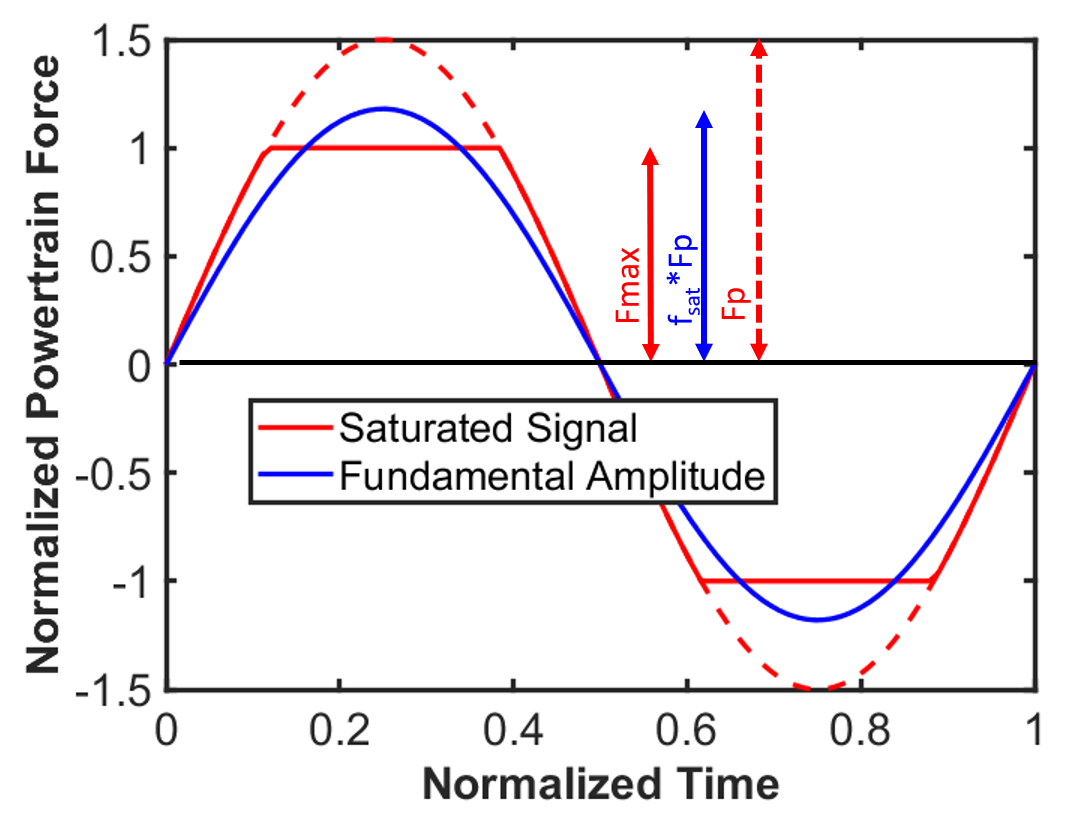
\includegraphics[width=8.4cm]{ifacconf_latex/figs/sin-saturation-3.png}
    \caption{Plot of a saturated sinusoid with appropriate amplitdues labeled.}
    \label{fig:sat-sin}
\end{figure}
We consider a saturation control law of the form
\begin{equation}
    I_{L,sat}(t) = I_{max}\textrm{sat}(I_{L,temp}(t)/I_{max})
\end{equation}
where $\textrm{sat}$ is the saturation function, $I_{L,temp}(t)$ is the time domain output of a standard linear impedance controller $I_{L,temp} = \frac{V_{L,sat}}{Z_C}$, stored temporarily in the controller's memory and never physically realized. Even though the relationship between $I_{L,temp}$ and $V_{L,sat}$ is linear, the temporary current $I_{L,temp}$ is not equal to $ I_L$ the current from a system with a linear controller, because $V_{L,sat} \neq V_L$. 

The waveform $I_{L,sat}(t)$ will be close to a saturated sinusoid, although not exact due to nonlinearities. Specifically, $I_{L,sat}(t)$ will inevitably contain harmonics due to saturation, shown as the orange arrow exiting the saturation block in Fig.~\ref{fig:block-diagram-nonlinear} (b). Those harmonics act as forces on the WEC and, due to the low pass nature of the effective mass-spring-damper dynamics, are substantially reduced but not eliminated in the velocity signal. The harmonics in velocity create harmonics in the voltage and thus harmonics in the hypothetical current before saturation $I_{L,temp}(t)$. Thus, $I_{L,sat}$ will have some small additional harmonics in addition to those of a saturated sinusoid, and here we neglect them due to the plant's low pass behavior. Sections (c) and (d) of Fig.~\ref{fig:block-diagram-nonlinear} both show this assumption as a green arrow exiting the controller block.

Section (c) is the standard describing function method, which uses the fundamental of the saturated current signal, and (d) is the higher order describing function from \cite{nuij_higher-order_2006}, which uses higher harmonics of the saturated current signal.
\begin{figure*}
    \centering
    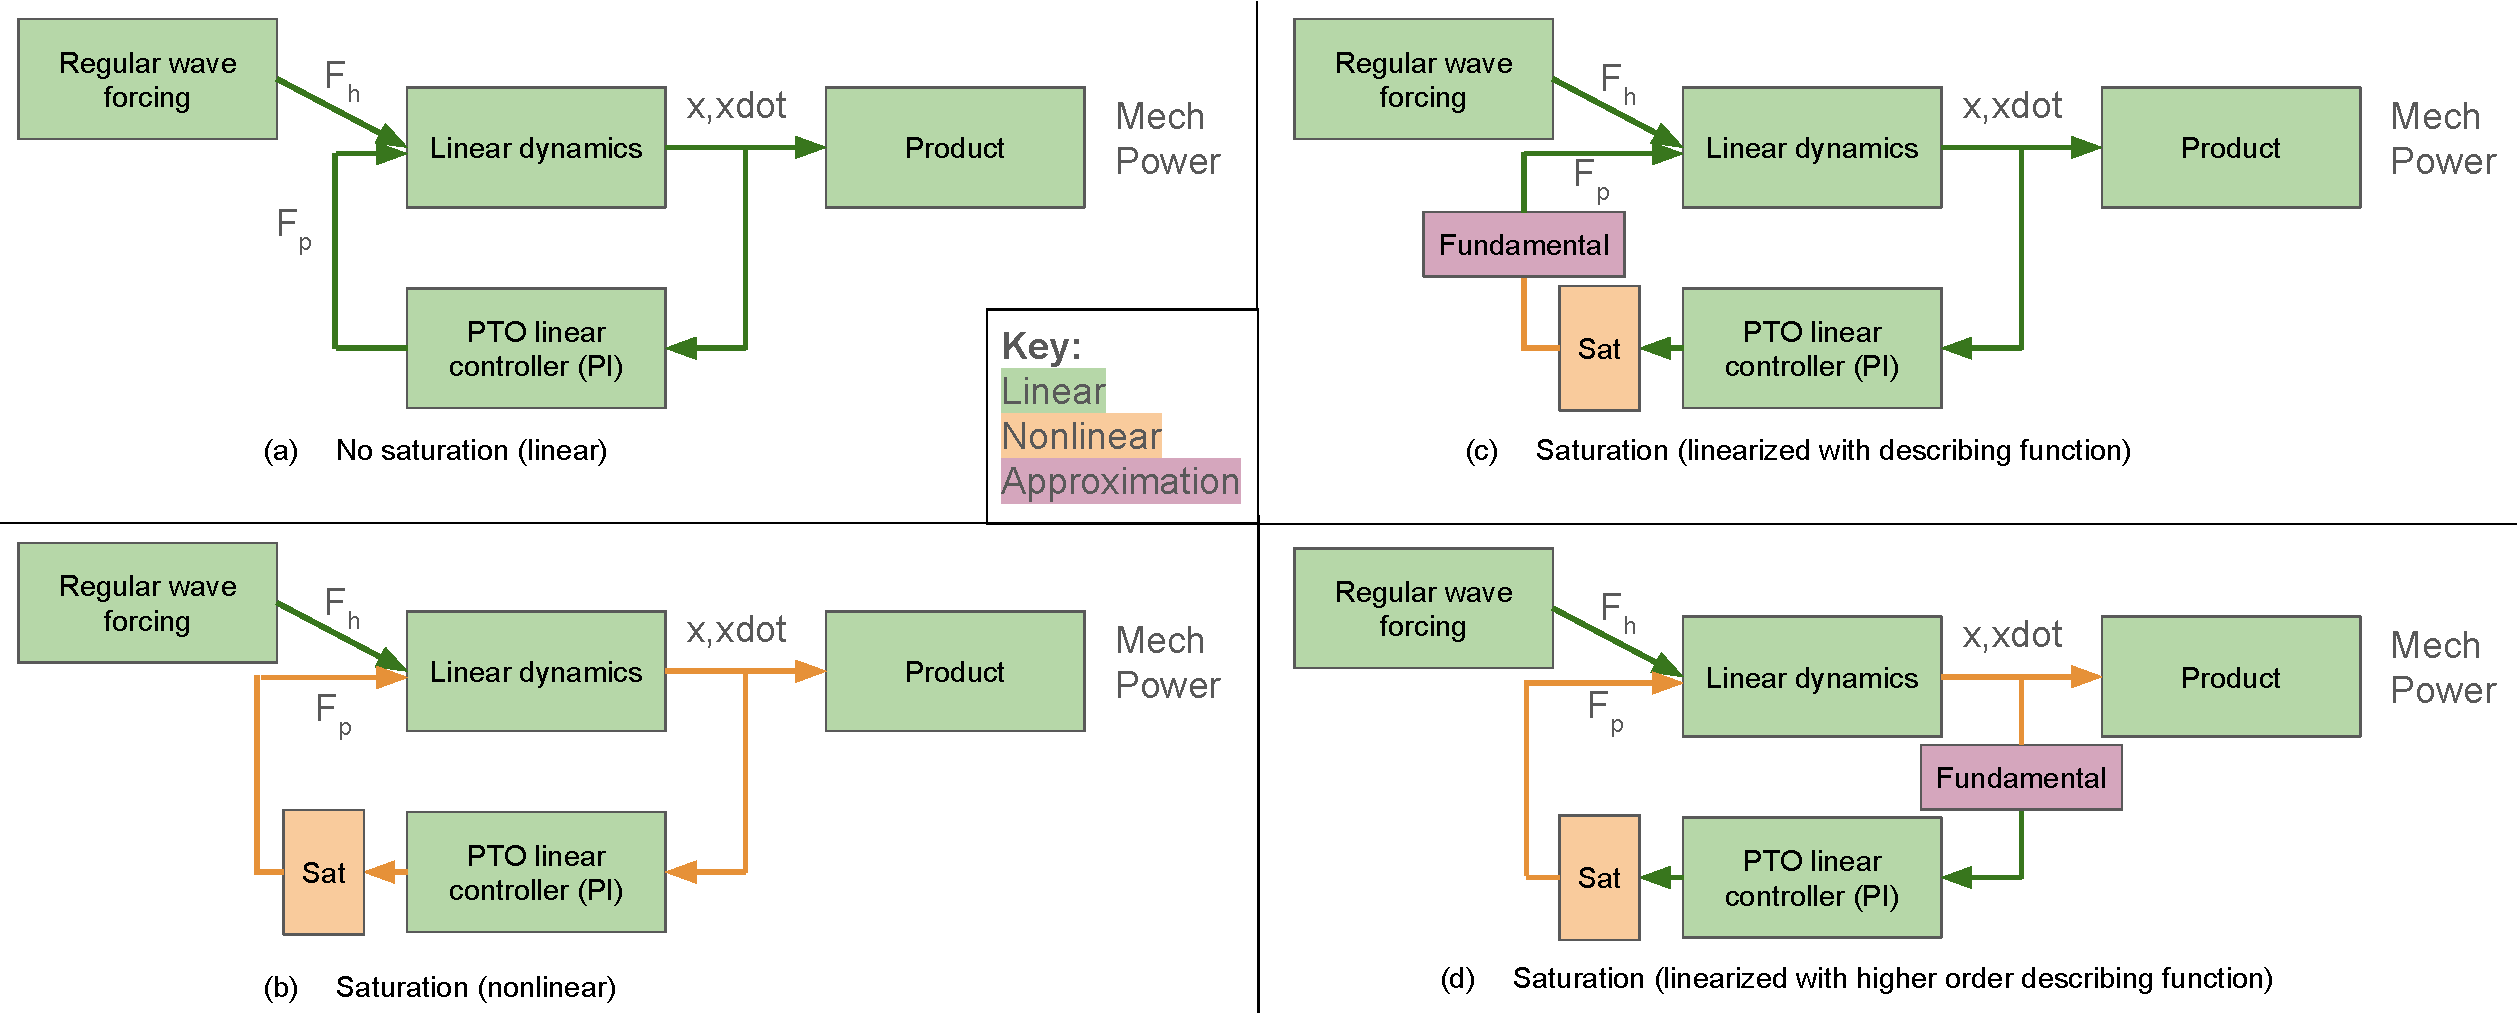
\includegraphics[width=18.2cm]{ifacconf_latex/figs/IFAC CAMS describing function block diagram.pdf}
    \caption{Block diagram illustration of describing functions used to linearize a wave energy saturation nonlinearity. Mechanical power is shown to keep the diagram simple, but the same concept applies to electrical power.}
    \label{fig:block-diagram-nonlinear}
\end{figure*}
The derivations immediately to follow preserve the higher current harmonics to enable higher order describing functions. %, while section \ref{sec:neglect-harmonics} uses standard describing functions for simplicity.
 Assuming a sinusoidal temporary current signal, we can decompose the saturated sinusoid current signal into the sum of the fundamental and higher harmonics: 
\begin{equation}
    I_{L,sat}(t) \approx \sum_n |I_{L,sat,n}| \sin(n \omega t + \psi)
\end{equation} where $\psi$ is the same phase as $I_{L,temp}(t)$ had. The amplitude of the $n$th current harmonic $|I_{L,sat,n}|$ is defined equal to $f_{sat,n} |I_{L,temp}|$, where $f_{sat,n}$ is a saturation factor compared to the temporary unsaturated current amplitude $|I_{L,temp}|$.
\begin{equation}\label{f-sat-i-defn}
    f_{sat,n} = \frac{|I_{L,sat,n}|}{|I_{L,temp}|} = \frac{|I_{L,sat,n}||Z_C|}{|V_{L,sat}|}
\end{equation}
To find $f_{sat,n}$, we can apply the describing function technique, leveraging Fourier analysis of a saturated sin wave to get an equivalent linear transfer function for the nonlinear saturation block, shown in (\ref{eq:f-sat-desc-fcn}), where $\theta = n \sin^{-1}\frac{I_{max}}{|I_{L,temp}|} $.
\begin{figure*}[htbp]
\begin{equation}\label{eq:f-sat-desc-fcn}
    f_{sat,n} =
\begin{cases}
1 & \quad |I_{L,temp}| \leq I_{max} ~\And~ n = 1\\
0 & \quad |I_{L,temp}| \leq I_{max} ~\And~ n \neq 1 \\
\frac{2}{\pi} \left(\frac{I_{max}}{|I_{L,temp}|}\sqrt{1 - \left(\frac{I_{max}}{|I_{L,temp}|}\right)^2} + \theta \right) & \quad |I_{L,temp}| > I_{max} ~\And~ n = 1 \\ 
0 & \quad |I_{L,temp}| > I_{max} ~\And~ n = 2,4,6,... \\
\frac{4}{\pi} \frac{1}{n (n^2 - 1)} \left( n \sqrt{1 - (\frac{I_{max}}{|I_{L,temp}|})^2}\sin(\theta) - \frac{I_{max}}{|I_{L,temp}|}\cos(\theta) \right) & \quad |I_{L,temp}| > I_{max} ~\And~ n = 3,5,7,...
\end{cases}
\end{equation}
\end{figure*}
This equation is depicted graphically in Fig.~\ref{fig:desc-fcn} for the first 7 harmonics. As the amount of saturation increases, the fundamental amplitude decreases, and the higher harmonics become more prominent. The limit for large $\frac{|I_{L,temp}|}{I_{max}}$ is a square wave.

\begin{figure}[htbp!]
    \centering
    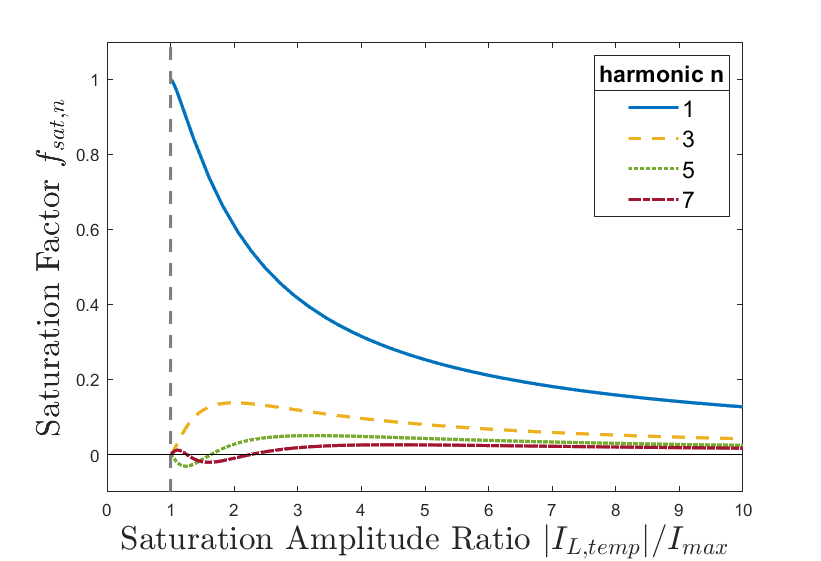
\includegraphics[width=8.4cm]{ifacconf_latex/figs/fsat3.png}
    \caption{Harmonic ratios $\frac{f_{sat,n}}{f_{sat,1}}$ as a function of the saturation amplitude ratio $\frac{|I_{L,temp}|}{I_{L,max}}$, for n = 1, 3, 5, and 7. All even harmonics are zero, and higher frequency harmonics have smaller amplitudes, which aligns with expectations.}
    \label{fig:desc-fcn}
\end{figure}

Consequently, at each harmonic frequency $n$, the saturation block can be approximated by an equivalent gain multiplier $f_{sat,n}$, such that the equivalent load impedance is $Z_L = Z_C / f_{sat,n}$ rather than $Z_L = Z_C$ as in the linear unsaturated case. This makes the nondimensional impedance for the $n$th harmonic $z_n = Z_C  / (f_{sat,n} Z_{th}^*)$. %This multiplier must be calculated to enforce $f_{sat,n}$ to the desired level. The gain multiplier $m_n$ does not equal the current saturation factor $f_{sat,n}$ because $V_{L,sat} \neq V_L$. 
Now we have a quasi-linear system, where the response is the sum of linear responses at different frequencies:
\begin{equation}
    \overline{P}_L = \Sigma_{n} P_{L,n}(z_n)
\end{equation}

% Because the plant is linear, each voltage harmonic will be a linear transformation of the current harmonics.  This means that the current created by the saturated controller can be approximated by a sum of scaled-down responses to unsaturated controllers:
% \begin{equation}\label{m-sat-intro}
% \begin{aligned}
%     \frac{|I_{L,sat,n}|}{|X_{sat,i}|} &\approx m_{sat,i} \frac{|F_{p,i}|}{|X_i|} = m_{sat,i} \sqrt{ (B_p i \omega)^2 + K_p^2} \\
%     I_{L,sat}(t) &\approx \sum_i m_{sat,i} \sqrt{ (B_p i \omega)^2 + K_p^2} ~|X_{sat,i}| \sin(i \omega t + \psi) \\
%     &\approx \sum_i m_{sat,i} (B_p \dot{x}_{sat,i} + K_p x_{sat,i} )
% \end{aligned}
% \end{equation}
% Applied to the full system dynamic response:
% \begin{equation}
%     \sum_i \left[ m \ddot{x}_{sat,i} + (B_h+m_{sat,i}B_p) \dot{x}_{sat,i} + (K_h + m_{sat,i}K_p) x_{sat,i} \right] \approx F_h \sin(\omega t)
% \end{equation}

%\subsection{Neglecting Higher Harmonics}\label{sec:neglect-harmonics}
Optionally, a reasonable approximation is to only consider $f_{sat,1}$ the fundamental current harmonic, as in Fig.~\ref{fig:block-diagram-nonlinear} (c). Because the plant is essentially a second order low pass filter, the higher harmonics are attenuated and contain little energy. %In this section, we make this additional approximation and use $f_{sat}$ to refer to and $f_{sat,1}$.

% The new dynamics are fully linear:
% \begin{equation}
%     m \ddot{x}_{sat} + (B_h+m_{sat}B_p) \dot{x}_{sat} + (K_h + m_{sat}K_p) x_{sat} \approx F_h \sin(\omega t)
% \end{equation}

% The gain multiplier $m_{sat}$ must be calculated from $f_{sat}$ such that the resulting saturated powertrain force is a factor $f_{sat}$ times the unsaturated powertrain force. From \eqref{f-sat-i-defn} and \eqref{m-sat-intro}, we have:
% \begin{equation} \label{eq:force-sat}
%     m_{sat} = f_{sat} \frac{|X|} {|X_{sat}|}
% \end{equation} 

%Design takeaway: force saturation will have the least impact on energy generation when the excitation frequency equals the uncontrolled natural frequency (pure hydrodynamic response) $\omega_{n,u}$. For typical hydrodynamic coefficients, excitation frequencies higher than $\omega_{n,u}$ abruptly result in less energy, and excitation frequencies lower than $\omega_{n,u}$ more gradually result in less energy. This suggests that for force-limited systems, it may make sense to design $\omega_{n,u}$ to be higher than it would be in an unsaturated system, to avoid the steep dropoff in energy at the ocean excitation frequencies. This is very promising because $\omega_{n,u} = \sqrt{\frac{K_h}{m}}$, and lowering the mass would achieve the desired increase in $\omega_{n,u}$ while also decreasing structural costs.

%\subsubsection{Including higher harmonics}
%Todo. Use the expression for $f_{sat,n}$ for i=3,5,7... in \eqref{f-sat-desc-fcn} to approximate the energy in the higher harmonics.

\subsection{Limitations}
The main limitation of the describing function is that it only applies to regular waves. The saturated sinusoid shape of the force waveform relies on a sinusoidal voltage wave. Real waves come from a broadband spectrum and are irregular. It remains to be tested how accurate the results are for irregular waves. Even for regular waves, describing functions still are approximations that rely on the low pass filter behavior of the WEC. For WECs that are broadband, such as small WECs, this assumption may be poor. Future work includes a full error analysis of the describing functions compared to a fully nonlinear simulation.

\section{Sensitivities}\label{sec:sensitivities}
Section \ref{sec:linear} and \ref{sec:nonlinear} will now be combined to yield overall sensitivity results. In a realistic WEC, perfect impedance matching may be possible in small waves, but above a certain threshold the generator's maximum force will be reached and a linear impedance mismatch or a nonlinear saturation strategy can be employed to extract as much energy as possible while respecting the constraint.

For simplicity, we consider the $\alpha=0$ case in Fig.~\ref{fig:sensitivity}, corresponding to $Z_{th}$ purely real (resistive) and $Z_m$ purely imaginary (reactive). In a matched controller, power varies quadratically with the excitation force $F_e$ from (\ref{eq:matched-values}) and (\ref{eq:thevenin}). For a linear impedance mismatch, \eqref{eq:optimal-vi} indicates that the current ratio equals $1 - \Gamma$. Plugging in \eqref{eq:ratio-power} and \eqref{eq:matched-values} yields:
\begin{equation}
    \overline{P}_L = \left( 1 - \left(1 - \frac{2 \Re(Z_{th}) I_{max}}{|V_{th}|}\right)^2 \right) \frac{|V_{th}|^2}{8 \Re(Z_{th})}
\end{equation}
Simplifying and setting all constants to enforce a normalized power of $1$ at $F_e=1$ (red marker in This is shown in Fig.~\ref{fig:sensitivity}) yields that the power scales linearly with $F_e$. Meanwhile, a nonlinear saturation strategy can provide a factor of up to $4/\pi$ larger fundamental, which means that it can achieve perfect impedance matching up until $F_e=\frac{4}{\pi}$ (blue marker in Fig.~\ref{fig:sensitivity}.) while also having a larger linear slope in the regions where it cannot achieve perfect matching. The describing function can quantify the power for larger $F_e$. This analysis allows designers to carefully select their largest wave for which impedance matching is possible, which will likely be much lower than the largest operational wave, because impedance mismatch can provide value at these points.
\begin{figure}[htbp!]\
    \centering
    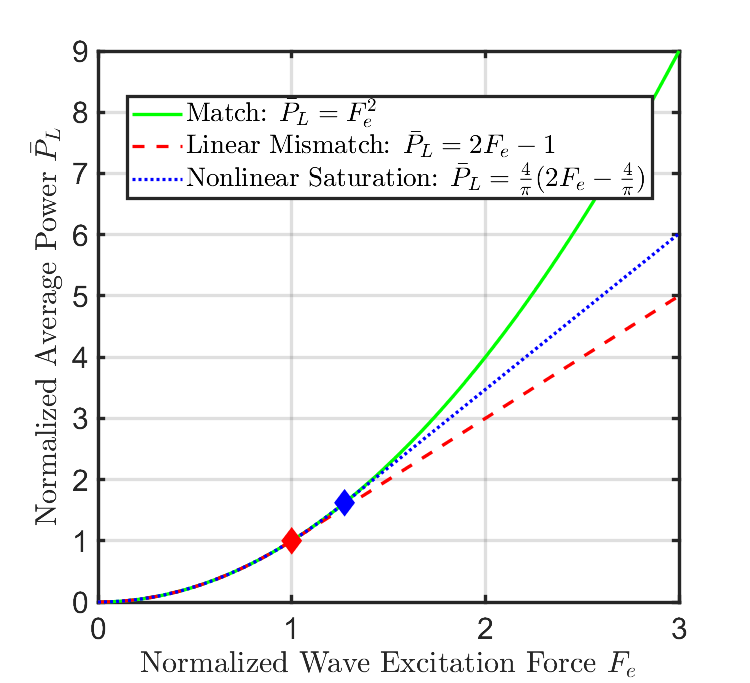
\includegraphics[width=8.4cm]{ifacconf_latex/figs/sensitivity-plot.png}
    \caption{Comparison of the power versus excitation force for three controller types. The matched controller does not limit the generator force, while the other two do.}
    \label{fig:sensitivity}
\end{figure}
%The generator is characterized by its maximum current, operating voltage, maximum displacement, resistance, and inductance. The current, voltage, and inductance dictate the generator's torque speed curve, typically considered its primary performance characteristic. The curve 
%is pictured in Fig.~\ref{fig:ts-curve} and consists of a thermally-limited constant torque at low speeds (current-limited region) and a decreasing torque at high speeds when the back EMF voltage approaches that of the drive (voltage-limited region). The maximum displacement is an important machine sizing characteristic for linear generators, and can become relevant for rotational powertrains with buoy kinematic constraints. Finally, the resistance also affects the efficiency of the machine through (\ref{eq:effic}). A generator's size, and therefore cost, scales with its maximum torque $\tau_{max}$ and rotational speed $\omega_{max}$ for rotary generators, and maximum force $F_{max}$, velocity $\dot{x}_{max}$, and displacement $x_{max}$ for linear generators. Therefore, it is useful to express the power production as a function of these constraints.

%\subsection{Dimensional Generator Sizing Implications}
%For comparison, we use cost values equal to that of a previous case study \cite{pena-sanchez_control_2022} that uses the pseudo-spectral method, a fully nonlinear numerical solver.

% \begin{equation}
%     CoS = 1.48 \cdot 10^3 \$/m
%     CoF = 0.1656 \$/N
%     C_{PTO} = 2.5 n_{gen} ( (L_{trans} + S_{max}) CoS + F_{trans} CoF) + C_{elec}
%     \bar{LCOE} = C_{PTO} / EP
% \end{equation}

\section{Conclusion}
This work presented an analytical framework for handling WEC generator force (current) constraints. First, the linear theory was reviewed, and key relationships for an impedance-mismatched Thévenin-equivalent circuit were visualized using Smith charts and Pareto fronts. Then, the specific dynamics for wave energy were introduced, and the implications of the nondimensional mechanical impedance and inductance on the Thévenin phase parameter $\alpha$ were highlighted. Next, describing function theory was introduced, with a description of where the nonlinearity is and how the low pass nature of the plant justifies neglecting higher harmonics. Finally, the two sections were combined together to demonstrate sensitivity to force limit under different control assumptions. 

A variety of extensions provide avenues for future work. The framework articulated here for force (current) constraints could easily be extended to other constraints, for example position, velocity, or phase voltage, by multiplying the ratios in (\ref{eq:ratios}) by the appropriate transfer function. Because these describing functions rely on a saturated-sin shape, they are not well-suited for examining two simultaneous constraints due to the overlapping nonlinearities, although the error remains to be quantified. The effect of irregular waves and frequency-dependent dynamics can likewise be investigated. In the context of WEC techno-economic optimization, the sensitivities should be coupled with a full generator model to inform the best design tradeoffs of power performance and machine size given realistic cost models. 

The analytical nature of this work provides intuition and computational speed for early-stage design or large-scale coupled optimization as needed. It does not take the place of numerical optimization such as the pseudo-spectral method, which can capture constraints fully nonlinearly, but still provides a relevant contribution to the field. For example, these analytical approximations could be used as the initial guess in a numerical optimization scheme to accelerate convergence. Finally, the general results related to impedance mismatch and signal limits can apply to many other domains of engineering that use impedance matching, such as circuits and robotics. 

The code for this work is available open-source at \url{https://github.com/symbiotic-engineering/IFAC_CAMS_2024/}.

%\begin{ack}
%Place acknowledgments here.
%\end{ack}

\bibliography{ifacconf_latex/references}

% \appendix
% \section{Ratios in terms of $z$}    % Each appendix must have a short title.
% Here, (\ref{eq:ratios}) is rewritten in terms of the impedance ratio $z$:
% \begin{equation}\label{eq:ratios-z}
% \begin{aligned}
%      \frac{\overline{P}_L}{\overline{P}_L^m} &= \frac{4 \Re(z)}{|z|^2 + 2 \Re(z) + 1} \\
%      \frac{|V_L|}{|V_L^m|} &= \frac{2 |z|}{\sqrt{(1+\alpha^2)(|z|^2+1) + 2(1-\alpha^2)\Re(z) + 4 \alpha \Im(z)  }} \\
%      \frac{|I_L|}{|I_L^m|} &= \frac{2}{\sqrt{(1+\alpha^2)(|z|^2+1) + 2(1-\alpha^2)\Re(z) + 4 \alpha \Im(z)  }}
% \end{aligned}
% \end{equation}

\end{document}
